\chapter{NLP Ethics and Fairness}
\label{chp:fairness}

The previous chapter presented how users express themselves differently across demographic groups and introduced two user factor adaptation methods via the multitask learning framework. 
As described in Section~\ref{chap4:subsec:analysis}, demographic variations exist in language and
further impact on robustness of language models.
While the Section~\ref{chap4:sec:dem_exp} shows that the demographic variations in language provide opportunities to improve document classification performance, the demographic variations may cause that the trained models may discriminate to some demographic groups than the others.

Recent research raises concerns that document classification models can be discriminatory and can perpetuate human biases~\cite{dixon2018measuring, kiritchenko2018examining, park2018reducing, garg2019counterfactual, borkan2019nuanced}.
\textit{Fairness}-aware classifiers aim to provide fair, non-discriminatory outcomes towards people or groups of people based on their demographic attributes, such as gender or race. 
Fairness has been defined in different ways~\cite{hardt2016equality}; for the document classification task, existing research~\cite{dixon2018measuring, kiritchenko2018examining, park2018reducing, garg2019counterfactual, heindorf2019debiasing} has focused on \textit{group fairness}~\cite{chouldechova2018frontiers}, under which document classifiers are defined as biased if the \textit{classifiers perform better for documents of some groups than for documents of other groups}.

This chapter will examine impacts of demographic variations in language for document classifiers in the perspectives of NLP ethics and fairness and show a standard domain adaptation method can generally reduce the demographic bias of document classifiers.
This chapter builds on material from \cite{huang2020multilingual}.

This chapter first presents a multilingual hate speech dataset with author-level demographic annotations (Section~\ref{chap5:sec:mul_data}). 
We combine previously published corpora labeled for Twitter hate speech recognition in English~\cite{waseem2016hateful,waseem2016you,founta2018large}, Italian~\cite{sanguinetti2018italian}, Polish~\cite{ptaszynski2017learning}, Portuguese~\cite{fortuna2019hierarchically}, and Spanish~\cite{basile2019semeval}, and publish this multilingual data augmented with author-level demographic information for four attributes: race, gender, age and country.
The demographic factors are inferred from user profiles, which are independent from text documents, the tweets.
Section~\ref{chap5:subsec:analysis} will take an exploratory study on the language variations across demographic groups on the English dataset.
To better understand how the demographic variations impact fairness of document classifiers, the section examines two questions from multiple language features:
\begin{itemize}
    \item Are Demographic Factors Predictable in Documents?
    \item Do Demographic Groups Express Document Categories Differently?
\end{itemize}
Section~\ref{chap5:sec:fair_eval} then experiments with four classification models to establish baseline levels of this corpus and evaluate the fairness performance of those document classifiers.
Finally, Section~\ref{chap5:sec:adaptation} handles each demographic attribute as domains (female vs. male domain); and apply a domain adaptation method~\cite{daume2007frustratingly} to debias document classifiers.
The proposed adaptation approach requires author demographic factors at training time but not at test time, where we learn domain independent document representations to be invariant towards demographic language variations.
The experiments show that the end-to-end domain adaptation models can outperform comparable document classification baselines on both general and fairness evaluation metrics.

\section{Introduction}


While document classification models should be objective and independent from human biases in documents, research have shown that the models can learn human biases and therefore be discriminatory towards particular demographic groups~\cite{dixon2018measuring,borkan2019nuanced,sun2019mitigating}.
The goal of \textit{fairness-aware} document classifiers is to train and build non-discriminatory models towards people no matter what their demographic attributes are, such as gender and ethnicity.
Existing research~\cite{dixon2018measuring,kiritchenko2018examining,park2018reducing,garg2019counterfactual,borkan2019nuanced} in evaluating fairness of document classifiers focus on the \textit{group fairness}~\cite{chouldechova2018frontiers}, which refers to every demographic group has equal probability of being assigned to the positive predicted document category.

However, the lack of original author demographic attributes and multilingual corpora bring challenges towards the fairness evaluation of document classifiers.
First, the datasets commonly used to build and evaluate the fairness of document classifiers obtain derived synthetic author demographic attributes instead of the original author information.
The common data sources either derive from Wikipedia toxic comments~\cite{dixon2018measuring,park2018reducing,garg2019counterfactual} or synthetic document templates~\cite{kiritchenko2018examining,park2018reducing}.
The Wikipedia Talk corpus\footnote{\url{https://figshare.com/articles/Wikipedia_Detox_Data/4054689}}~\cite{wulczyn2017ex} provides demographic information of annotators instead of the authors, Equity Evaluation Corpus\footnote{\url{http://saifmohammad.com/WebPages/Biases-SA.html}}~\cite{kiritchenko2018examining} are created by sentence templates and combinations of racial names and gender coreferences.
While existing work~\cite{davidson2019racial,diaz2018addressing} infers user demographic information (white/black, young/old) from the text, such inference is still likely to cause confounding errors that impact and break the independence between demographic factors and the fairness evaluation of text classifiers.
Second, existing research in the fairness evaluation mainly focus on only English resources, such as age biases in blog posts~\cite{diaz2018addressing}, gender biases in Wikipedia comments~\cite{dixon2018measuring} and racial biases in hate speech detection~\cite{davidson2019racial}.
Different languages have shown different patterns of linguistic variations across the demographic attributes~\cite{johannsen2015cross,huang2019neural}, methods~\cite{zhao2017men,park2018reducing} to reduce and evaluate the demographic bias in English corpora may not apply to other languages. 
For example, Spanish has gender-dependent nouns, but this does not exist in English~\cite{sun2019mitigating}; and Portuguese varies across Brazil and Portugal in both word usage and grammar~\cite{maier2014language}.
The rich variations have not been explored under the fairness evaluation due to lack of multilingual corpora.
% discuss some corpora that used for hate speech detection
Additionally, while we have hate speech detection datasets in multiple languages~\cite{waseem2016hateful,sanguinetti2018italian,ptaszynski2017learning,basile2019semeval,fortuna2019hierarchically}, there is still no integrated multilingual corpora that contain author demographic attributes which can be used to measure group fairness.
%in the hate speech recognition task.
The lack of author demographic attributes and multilingual datasets limits research for evaluating classifier fairness and developing unbiased classifiers.



\section{Related Work}

\paragraph{Demographic biases in hate speech detector}
Language varies substantially across demographic groups, especially in online data~\cite{goel2016social, hinds2018demographic}. For example, sensitive words such as queer show higher frequency in toxic comments~\cite{dixon2018measuring}, and males are more likely to use the word \textit{weakness} in a negative way while females are more likely use it in a positive way~\cite{volkova2013exploring}. Such variations can affect hate speech detectors and lead to biased classifiers~\cite{sap2019risk, shah2020predictive} from multiple levels. First, annotation bias, annotators tend to annotate hate speech labels to the tweets that have African American words~\cite{sap2019risk}. Second, feature bias, the dissimilar demographic language usage in training and test sets can cause model discriminatory towards highly frequent features in some demographic groups~\cite{davidson2019racial}. Third, model bias, model can be sensitive to human discriminatory signals, such as gender pronoun and human names~\cite{kiritchenko2018examining}. 



\paragraph{Reduce biases in hate speech detector}
Debiasing document classifiers on hate speech related topics have been explored in the several demographic attributes, such as age~\cite{diaz2018addressing, gencoglu2020cyberbullying}, gender~\cite{dixon2018measuring, park2018reducing}, race~\cite{davidson2019racial, xia2020demoting}.
On the data level, \cite{dixon2018measuring, davidson2019racial} proposed data augmentation strategies that remove or replace racial and gender related tokens.
On model level, \cite{gencoglu2020cyberbullying} proposed a joint framework that optimizes classification models with fairness and label evaluation metrics, \cite{zhang2018mitigating, xia2020demoting} proposed adversarial training methods to mitigate unintended biases, and \cite{park2018reducing} explored using the debiased word embedding and fine-tuning to reduce the gender bias.

In this chapter, we propose a multilingual hate speech corpora that allows for evaluating author-level demographic bias of hate speech detector, and further propose a feature augmentation method to reduce demographic biases of document classification models.


\section{Data}
\label{chap5:sec:mul_data}

We assemble the annotated datasets for hate speech classification.
To narrow down the data sources, we limit our dataset sources to the unique online social media site, Twitter.
We have requested 16 published Twitter hate speech datasets, and finally obtained 7 of them in five languages.
By using the Twitter streaming API\footnote{\url{https://developer.twitter.com/}}, we collected the tweets annotated by hate speech labels and their corresponding user profiles in English~\cite{waseem2016hateful, waseem2016you,founta2018large}, Italian~\cite{sanguinetti2018italian}, Polish~\cite{ptaszynski2017learning}, Portuguese~\cite{fortuna2019hierarchically}, and Spanish~\cite{basile2019semeval}.
We binarize all tweets' labels (indicating whether a tweet has indications of hate speech), allowing to merge the different label sets and reduce the data sparsity.

Whether a tweet is considered hate speech heavily depends on who the speaker is; for example, whether a racial slur is intended as hate speech depends in part on the speaker's race~\cite{waseem2016hateful}.
Therefore, hate speech classifiers may not generalize well across all groups of people, and disparities in the detection offensive speech could lead to bias in content moderation~\cite{shen2018perception}.
Our contribution is to further annotate the data with user demographic attributes inferred from their public profiles,
thus creating a corpus suitable for evaluating author-level fairness for this hate speech recognition task across multiple languages.

\subsection{User Attribute Inference}
\label{chap5:subsec:infer}

We consider four user factors of age, race, gender and geographic location. For location, we inference two granularities, country and US region, but only experiment with the country attribute.
While the demographic attributes can be inferred through tweets~\cite{volkova2015inferring,davidson2019racial},
we intentionally exclude the contents from the tweets if they infer these user attributes, in order to make the evaluation of fairness more reliable and independent.
If users were grouped based on attributes inferred from their text, then any differences in text classification across those groups could be related to the same text. 
Instead, we infer attributes from public user profile information (i.e., description, name and photo).

\paragraph{Age, Race, Gender.}
We infer these attributes from each user's profile image by using Face++ (\url{https://www.faceplusplus.com/}),
a computer vision API that provides estimates of demographic characteristics.
Empirical comparisons of facial recognition APIs have found that Face++ is the most accurate tool on Twitter data~\cite{jung2018assessing} and works comparatively better for darker skins~\cite{buolamwini2018gender}.
For the gender, we choose the binary categories (male/female) by the predicted probabilities.
We map the racial outputs into four categories: Asian, Black, Latino and White.
We only keep users that appear to be at least 13 years old, and we save the first result from the API if multiple faces are identified.
We experiment and evaluate with binarization of race and age with roughly balanced distributions (white and nonwhite, $\leq$ median vs. elder age) to consider a simplified setting across different languages, since race is harder to infer accurately.

\paragraph{Country.}
The country-level language variations can bring challenges that are worth to explore.
We extract geolocation information from users whose profiles contained either numerical location coordinates or a well-formatted (matching a regular expression) location name. 
We fed the extracted values to the Google Maps API (\url{https://maps.googleapis.com}) to obtain structured location information (city, state, country).
We first count the main country source and then binarize the country to indicate if a user is in the main country or not. 
For example, the majority of users in the English are from the United States (US), therefore, we can binarize the country attributes to indicate if the users are in the US or not.

% Data stats
\subsection{Corpus Summary} 

\begin{table}[htp]
\centering
\begin{tabular}{c||cccc}
Language & Users & Docs & Tokens & HS Ratio \\\hline\hline
English & 64,067 & 83,077 & 20.066 & .370 \\
Italian & 3,810 & 5,671 & 19.721 & .195 \\
Polish & 86 & 10,919 & 14.285 & .089 \\
Portuguese & 600 & 1,852 & 18.494 & .205 \\
Spanish & 4,600 & 4,831 & 19.199 & .397
\end{tabular}
\caption{Statistical summary of multilingual corpora across English, Italian, Polish, Portuguese and Spanish. We present number of users (Users), documents (Docs), and average tokens per document (Tokens) in the corpus, 
plus the label distribution (HS Ratio, percent of documents labeled positive for hate speech).}
\label{chap5:tab:corpus}
\end{table}

We show the corpus statistics in Table~\ref{chap5:tab:corpus} and summarize the full demographic distributions in Table~\ref{chap5:tab:user}. 
The binary demographic attributes (age, country, gender, race) can bring several benefits. 
First, we can create comparatively balanced label distributions. 
We can observe that there are differences in the race and gender among Italian and Polish data, while other attributes across the other languages show comparably balanced demographic distributions.
Second, we can reduce errors inferred from the Face++ on coarse labels.
Third, it is more convenient for us to analyze, conduct experiments and evaluate the group fairness of document classifiers.


\begin{table*}[htp]
\centering
\begin{tabular}{c||cc|cc|cc|cc}
Language & \multicolumn{2}{c|}{Age} & \multicolumn{2}{c|}{Country} & \multicolumn{2}{c|}{Gender} & \multicolumn{2}{c}{Race} \\\hline\hline
\multirow{2}{*}{English} & Mean & Median & US & non-US & Female & Male & White & non-White \\
 & 32.041 & 29 & .599 & .401 & .499 & .501 & .505 & .495 \\\hline
\multirow{2}{*}{Italian} & Mean & Median & Italy & non-Italy & Female & Male & White & non-White \\
 & 44.518 & 43 & .778 & .222 & .307 & .692 & .981 & .018 \\\hline
\multirow{2}{*}{Polish} & Mean & Median & Poland & non-Poland & Female & Male & White & non-White \\
 & 39.245 & 38 & .795 & .205 & .324 & .676 & .895 & .105 \\\hline
\multirow{2}{*}{Portuguese} & Mean & Median & Brazil & non-Brazil & Female & Male & White & non-White \\
 & 29.635 & 26 & .437 & .563 & .569 & .431 & .508 & .492 \\\hline
\multirow{2}{*}{Spanish} & Mean & Median & Spain & non-Spain & Female & Male & White & non-White \\
 & 31.911 & 27 & .339 & .661 & .463 & .537 & .549 & .451
\end{tabular}
\caption{Statistical summary of user attributes in age, country, gender and race. For the age, we present both mean and median values in case of outliers. For the other attributes, we show binary distributions.}
\label{chap5:tab:user}
\end{table*}

Table~\ref{chap5:tab:corpus} presents different patterns of the corpus. 
The Polish data has the smallest users. 
This is because the data focuses on the people who own the most popular accounts in the Polish data~\cite{ptaszynski2017learning}, the other data collected tweets randomly.
And the dataset shows a much more sparse distribution of the hate speech label than the other languages.

Table~\ref{chap5:tab:user} presents different patterns of the user attributes. 
English, Portuguese and Spanish users are younger than the Italian and Polish users in the collected data.
And both Italian and Polish show more skewed demographic distributions in country, gender and race, while the other datasets show more balanced distributions.

\subsection{Demographic Inference Accuracy}

Image-based approaches will have inaccuracies, as a person's demographic attributes cannot be conclusively determined merely from their appearance. 
However, given the difficulty in obtaining ground truth values, we argue that automatically inferred attributes can still be informative for studying classifier fairness. 
If a classifier performs significantly differently across different groups of users, then this shows that the classifier is biased along certain groupings, even if those groupings are not perfectly aligned with the actual attributes they are named after. 
This subsection tries to quantify how reliably these groupings correspond to the demographic variables.


\begin{table}[th]
\centering
\begin{tabular}{c||c|c|c}
 & Age & Race & Gender \\ \hline
\multicolumn{4}{c}{Annotator Agreement} \\ \hline
Face++ & .80 & .80 & .98 \\ \hline
\multicolumn{4}{c}{Accuracy} \\ \hline
English & .86 & .90 & .94 \\ \hline
Italian & .82 & .96 & .98 \\ \hline
Polish & .88 & .96 & .98 \\ \hline
Portuguese & .82 & .78 & .92 \\ \hline
Spanish & .76 & .82 & .90 \\ \hline
Overall & .828 & .884 & .944 \\ 
\end{tabular}
\caption{Annotator agreement (percentage overlap) and evaluation accuracy for Face++.}
\label{chap5:tab:api_eval}
\end{table}

Prior research found that Face++ achieves 93.0\% and 92.0\% accuracy on gender and ethnicity evaluations~\cite{jung2018assessing}.
We further conduct a small evaluation on the hate speech corpus by a small sample of annotated user profile photos providing a rough estimate of accuracy while acknowledging that our annotations are not ground truth.
We obtained the annotations from the crowdsourcing website, Figure Eight (\url{https://figure-eight.com/}).
We randomly sampled 50 users whose attributes came from Face++ in each language.
We anonymize the user profiles and feed the information to the crowdsourcing website.
Three annotators annotated each user photo with the binary demographic categories.
To select qualified annotators and ensure quality of the evaluations, we set up 5 golden standard annotation questions for each language.
The annotators can join the evaluation task only by passing the golden standard questions.
We decide demographic attributes by majority votes and present evaluation results in Table~\ref{chap5:tab:api_eval}.
Our final evaluations show that overall the Face++ achieves averaged accuracy scores of 82.8\%, 88.4\% and 94.4\% for age, race and gender respectively.

\subsection{Privacy Considerations}
To facilitate the study of classification fairness, we publicly distributed this anonymized corpus with the inferred demographic attributes including both original and binarized versions.
To preserve user privacy, we will not publicize the personal profile information, including user ids, photos, geocoordinates as well as other user profile information, which were used to infer the demographic attributes.
We will, however, provide inferred demographic attributes in their original formats from the Face++ and Google Maps based on per request to allow wider researchers and communities to replicate the methodology and probe more depth of fairness in document classification.


\section{Language Variations across Demographic Groups}
\label{chap5:subsec:analysis}
% Motivation to explore the how they express differently
Demographic factors can improve the performances of document classifiers~\cite{hovy2015demographic}, and demographic variations root in language, especially in social media data~\cite{volkova2013exploring,hovy2015demographic}.
For example, language styles are highly correlated with authors' demographic attributes, such as age, race, gender and location~\cite{coulmas_2017,preoctiuc2018user}. Research~\cite{bolukbasi2016man,zhao2017men,garg2018word} find that biases and stereotypes exist in word embeddings, which is widely used in document classification tasks. For example, ``receptionist'' is closer to females while ``programmer'' is closer to males, and ``professor'' is closer to Asian Americans while ``housekeeper'' is closer to Hispanic Americans.

This motivates us to explore and test if the language variations hold in our particular dataset, how strong the effects are.
We do this in two perspectives, predictability and distance, from three levels, word, part-of-speech (POS) and topic.


\subsection{Are Demographic Factors Predictable in Documents?}
\label{chap5:subsec:pred}

We examine how accurately the documents can predict author demographic attributes from three different levels:
\begin{enumerate}
    \item Word-level. We extract TF-IDF-weighted 1-, 2-grams features.
    \item POS-level. We use Tweebo parser~\cite{kong2014dependency} to tag and extract POS features. We count the POS tag and then normalize the counts for each document.
    \item Topic-level. We train a Latent Dirichlet Allocation~\cite{blei2003latent} model with 20 topics using Gensim~\cite{rehurek2010software} with default parameters. Then a document can be represented as a probabilistic distribution over the 20 topics.
\end{enumerate}

We shuffle and split data into training (70\%) and test (30\%) sets.
We separately train three different logistic classifiers by the three levels of features.
We measure the prediction accuracy and show the absolute improvements of scores in Figure~\ref{chap5:fig:predictability}.

\begin{figure}[htp]
\centering
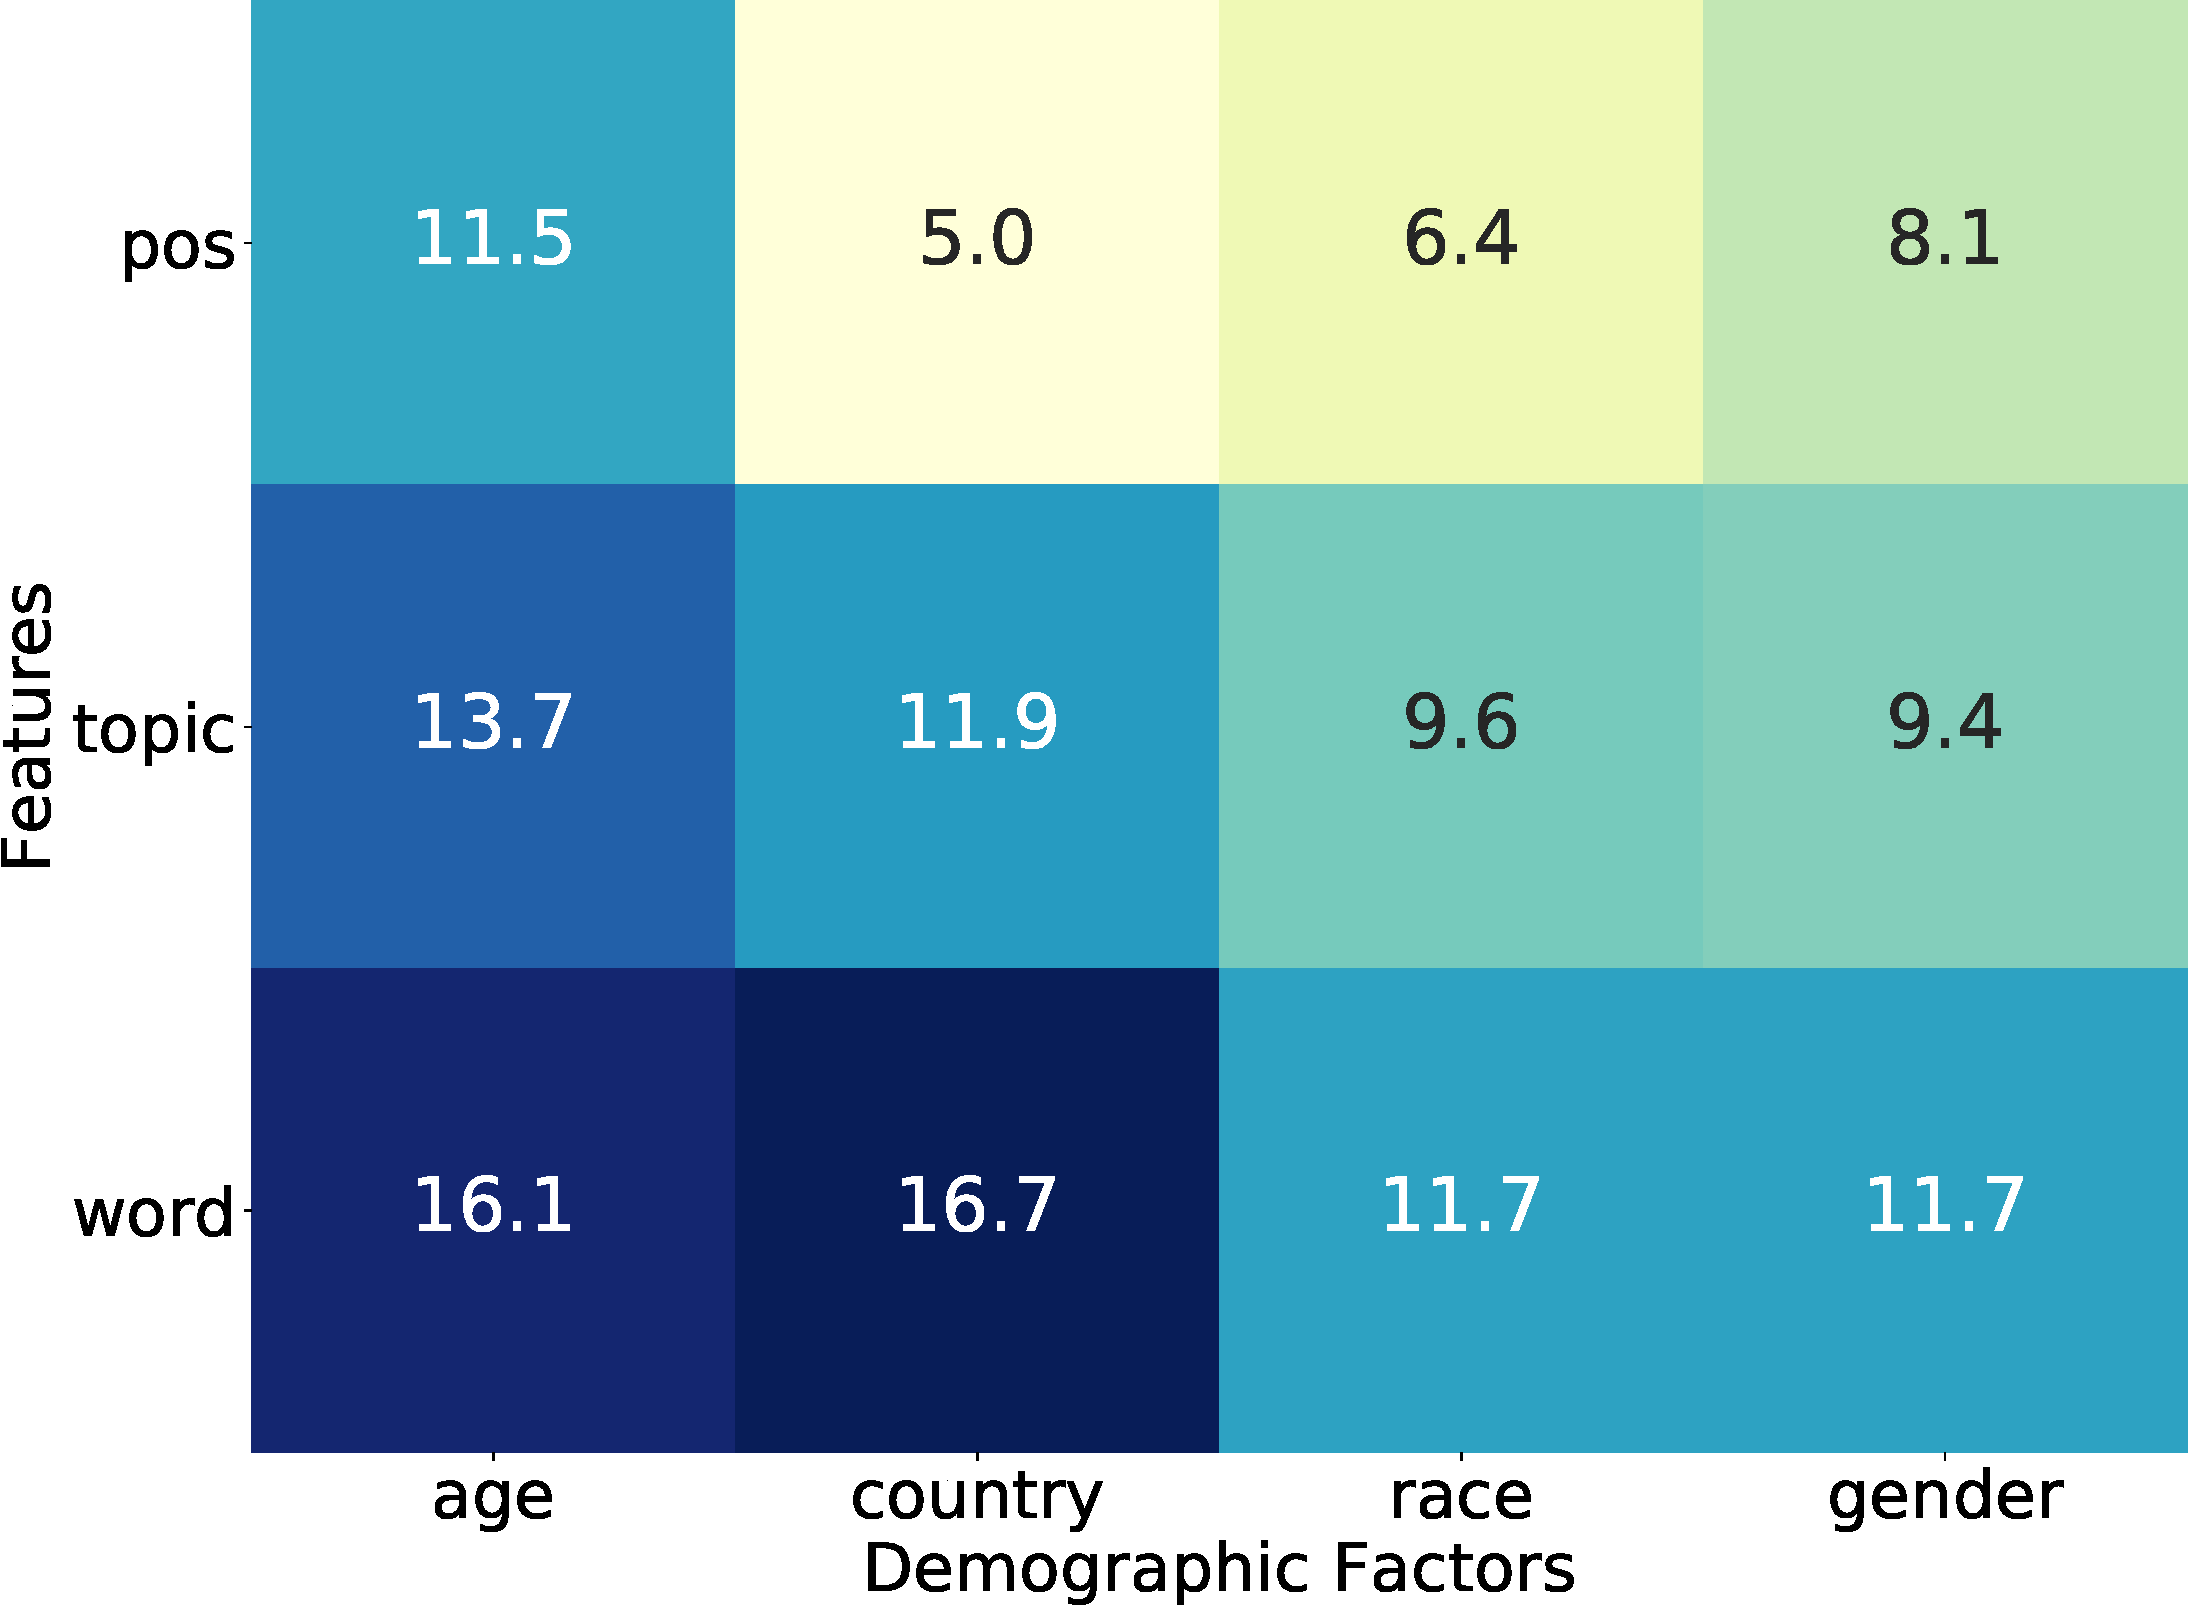
\includegraphics[width=0.55\textwidth]{images/chapter5/predictability.pdf}
\caption{Predictability of demographic attributes from language
data. We show the absolute percentage improvements in accuracy over majority-class baselines. The majority-class baselines of accuracy scores are either .500 for the binary prediction. The darker color indicates higher improvements and vice versa.}
\label{chap5:fig:predictability}
\end{figure}

The improved prediction accuracy scores over majority baselines suggest that language variations across demographic groups are encoded in the text documents. 
The results show that documents are the most predictable to the age attribute.
We can also observe that the word is the most predictable feature to demographic factors,
while the POS feature is least predictable towards the country factor.
These suggest there might be a connection between language variations and demographic groups.
This motivates us to further explore the language variations based on word features.
We rank the word features by mutual information classification~\cite{pedregosa2011scikit} and present the top 10 unigram features in Table~\ref{chap5:tab:features}.
The qualitative results show the most predictable word features towards the demographic groups and 
suggest such variations may impact extracted feature representations and further training document classifiers.


\begin{table*}[htp]
\centering
\resizebox{1\columnwidth}{!}{
    \begin{tabular}{cc||c}
    \multicolumn{2}{c||}{Demographic Attributes} & Top 10 Features of Demographic Attribute Prediction \\\hline\hline
    \multirow{2}{*}{Race} & White & nigga, fucking, ass, bro, damn, niggas, sir, moive, melon, bitches \\
     & Other & abuse, gg, feminism, wadhwa, feminists, uh, freebsd, feminist, ve, blocked \\\hline
    \multirow{2}{*}{Gender} & Female & rent, driving, tho, adorable, met, presented, yoga, stressed, awareness, me \\
     & Male & idiot, the, players, match, idiots, sir, fucking, nigga, bro, trump
    \end{tabular}
}
\caption{Top 10 predictable features of race and gender.}
\label{chap5:tab:features}
\end{table*}

% discuss the findings
The Table~\ref{chap5:tab:features} shows that when classifying hate speech tweets, the n-words and b-words are more significant correlated with the white instead of the other racial groups.
However, this shows an opposite view than the existing work~\cite{davidson2019racial}, which presents the two types of words are more significantly correlated with the black.
This can highlight the values of our approach that to avoid confounding errors, we obtain author demographic information independently from the user generated documents.


\subsection{Do Demographic Groups Express Document Categories Differently?}

Textual features, which are fundamental to build document classifiers, inherently vary across different demographic attributes, such as gender, age, location and political orientation~\cite{gao2015more,hinds2018demographic}.
Expressing differently between demographic groups to show the same sentiments will confuse document classifiers and lead to biased classifiers.
For example, balancing sensitive word features increase the biases of document classifiers~\cite{dixon2018measuring}.
Therefore, this motivates us to explore if textual features that are extracted for document classifiers vary across demographic groups.

To compare and measure demographic variations of textual features, we conduct comparisons on three different levels:

\paragraph{Word-level.} For each demographic group, we extract n-gram features (same feature sets as in the previous subsection) that are most associated with the document labels. With mutual information, we select the top 1,000 features for each group. Within each demographic attribute, we then calculate the percentage of overlap across different groups (e.g., males and females in gender factor): if $F_0$ is the set of top features for one factor and $F_1$ is the set of top features for another factor, the percent overlap is calculated as $|F_0 \cap F_1|/1000$.

\paragraph{POS-level.} For each demographic group, we extract and aggregate POS features (same feature sets as in the previous subsection). After normalizing the accumulated features, we can obtain POS representations for each demographic group. Within each demographic factor, we use Wasserstein distance to measure the distributional distance. Wasserstein distance or Earth Mover's distance~\cite{vallender1974calculation} is to measure the distributional differences between source and target domains in domain adaptation. In this study, we treat each demographic factor as a domain, and use the Wasserstein distance to measure demographic variations.

\paragraph{Topic-level.} For each demographic group, we use the trained topic model (same as in the previous subsection) to extract and calculate the average topic distribution across documents from that group. Then within each demographic factor, we measure language variations across demographic groups by Wasserstein distance. 

\begin{figure}[htp]
\centering
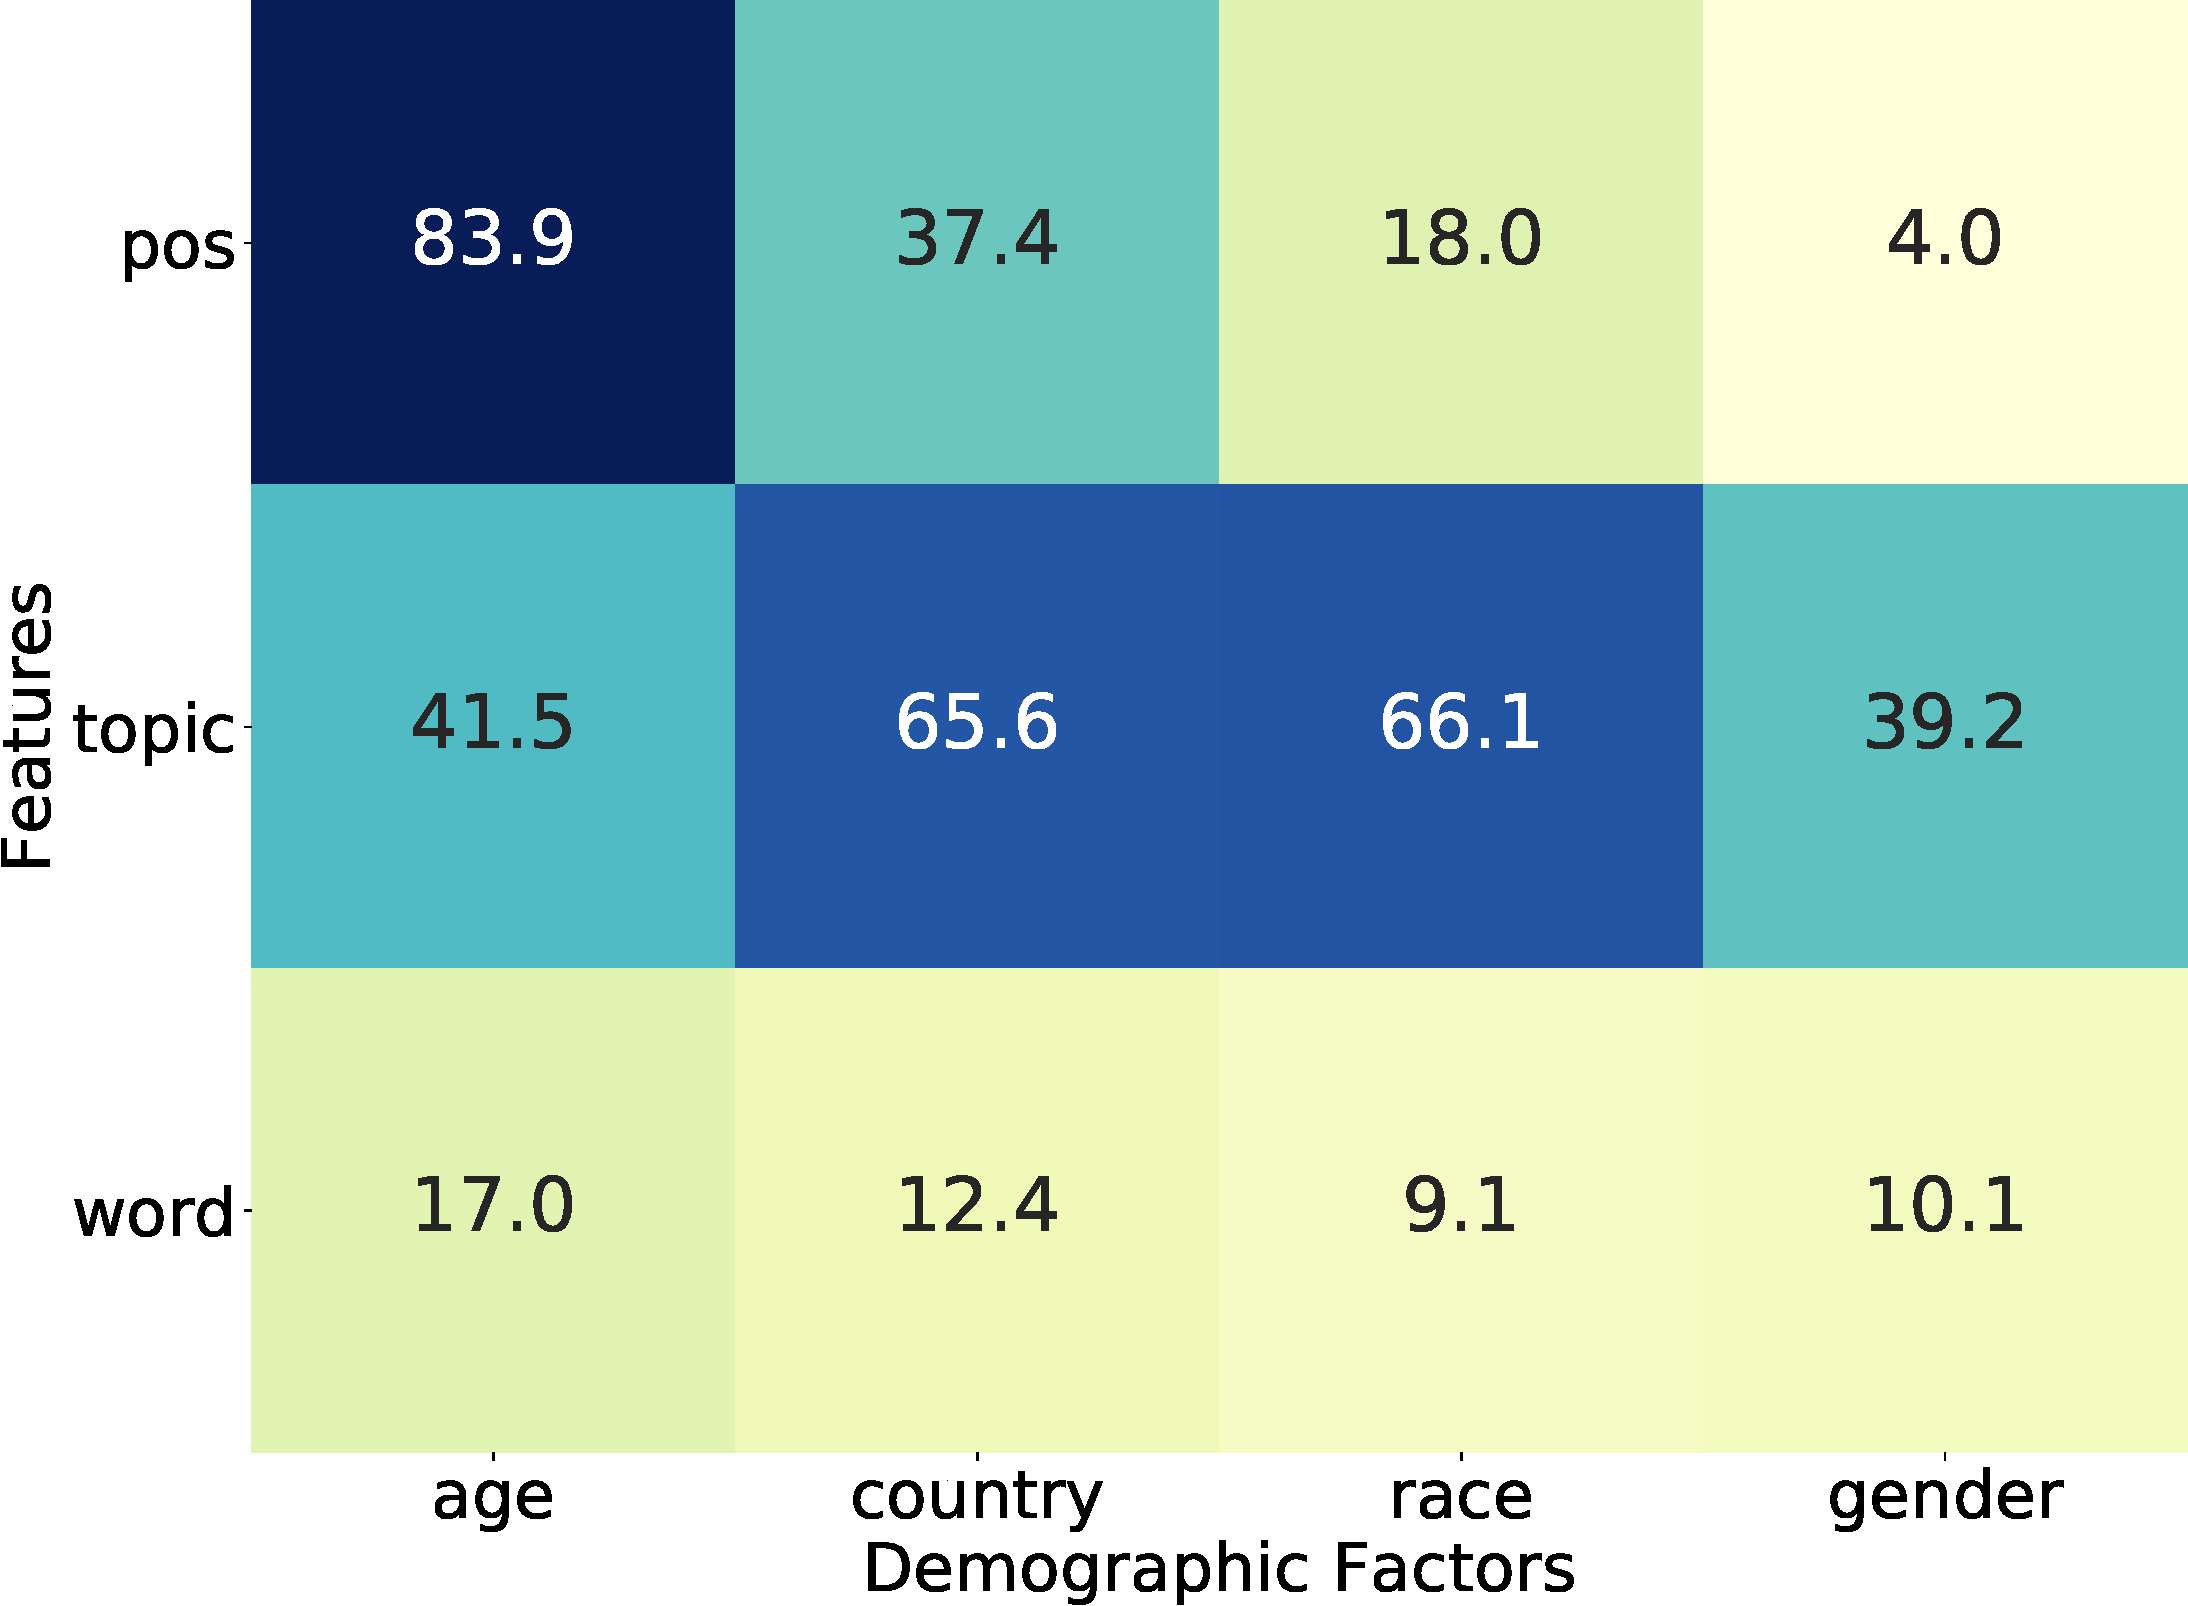
\includegraphics[width=0.55\textwidth]{images/chapter5/overlaps.pdf}
\caption{Language variations on how people express sentiment differently are calculated for each demographic factor. Darker color indicates more variations in expressing sentiments being classified.}
\label{chap5:fig:overlaps}
\end{figure}


To measure fairly expression variations, we randomly sample two groups of documents for each demographic factor as comparison sets. 
We calculate the overlaps and distances on the randomly sampled sets. 
We then compare percentage differences of the overlaps and distance scores between the demographic factors and the randomly selected sets: if $S_d$ is the overlap or distance score of one factor and $S_r$ is the score from the random comparison group, the percentage difference is calculated as $|S_d - S_r|/S_r$.
Results are visualized in Figure~\ref{chap5:fig:overlaps}. 
Higher percentage differences indicate higher variations across demographic groups express sentiments.
We can observe there are more variations in age from the topic and POS levels.


\section{Fairness Evaluation of Baseline Classifiers}
\label{chap5:sec:fair_eval}

Demographic variations root in documents, especially in social media data~\cite{volkova2013exploring,hovy2015demographic,johannsen2015cross}.
Such variations could further impact the performance and fairness of document classifiers.
In this study, we experiment four different classification models including logistic regression (LR), recurrent neural network (RNN)~\cite{chung2014empirical}, convolutional neural network (CNN)~\cite{kim2014convolutional} and Google BERT~\cite{devlin2019bert}.
We present the baseline results of both performance and fairness evaluations across the multilingual corpus.

\subsection{Data Preprocessing}
To anonymize user information, we hash user and tweet ids and then replace hyperlinks, usernames, and hashtags with generic symbols (URL, USER, HASHTAG).
Documents are lowercased and tokenized using NLTK~\cite{bird2004nltk}. 
The corpus is randomly split into training (70\%), development (15\%), and test (15\%) sets. 
We train the models on the training set and find the optimal hyperparameters on the development set before final evaluations on the test set. 
We randomly shuffle the training data at the beginning of each training epoch.



\subsection{Baseline Models}
We implement and experiment four baseline classification models. 
To compare fairly, we keep the feature size up to 15K for each classifier across all five languages.
We calculate the weight for each document category by $\frac{N}{N_l}$~\cite{king2001logistic}, where $N$ is the number of documents in each language and $N_l$ is the number of documents labeled by the category.
Particularly, for training BERT model, we append two additional tokens, ``[CLS]'' and ``[SEP]'', at the start and end of each document respectively.
For the neural models, we pad each document or drop rest of words up to 40 tokens.
We use ``unknown'' as a replacement for unknown tokens.
We initialize CNN and RNN classifiers by pre-trained word embeddings~\cite{mikolov2013distributed,godin2015multimedia,bojanowski2017enriching,deriu2017leveraging} and train the networks up to 10 epochs.

\paragraph{LR.} 
We first extract TF-IDF-weighted features of uni-, bi-, and tri-grams on the corpora, using the most frequent 15K features with the minimum feature frequency as 2. 
We then train a \texttt{LogisticRegression} from scikit-learn~\cite{pedregosa2011scikit}. 
We use ``liblinear'' as the solver function and leave the other parameters as default.

\paragraph{CNN.} 
We implement the Convolutional Neural Network (CNN) classifier described in~\cite{kim2014convolutional,zimmerman2018improving} by Keras~\cite{chollet2015keras}.
We first apply 100 filters with three different kernel sizes, 3, 4 and 5.
After the convolution operations, we feed the concatenated features to a fully connected layer and output document representations with 100 dimensions.
We apply ``softplus'' function with a l2 regularization with $.03$ and a dropout rate with $.3$ in the dense layer.
The model feeds the document representation to final prediction.
We train the model with batch size 64, set model optimizer as Adam~\cite{kingma2014adam} and calculate loss values by the cross entropy function.
We keep all other parameter settings as described in the paper~\cite{kim2014convolutional}.


\paragraph{RNN.}
We build a recurrent neural network (RNN) classifier by using bi-directional Gated Recurrent Unit (bi-GRU)~\cite{chung2014empirical,park2018reducing}.
We set the output dimension of GRU as 200 and apply a dropout on the output with rate $.2$.
We optimize the RNN with RMSprop~\cite{tieleman2012lecture} and use the same loss function and batch size as the CNN model.
We leave the other parameters as default in the Keras~\cite{chollet2015keras}.


\paragraph{BERT.}
BERT is a transformer-based pre-trained language model which was well trained on multi-billion sentences publicly available on the web~\cite{devlin2019bert}, which can effectively generate the precise text semantics and useful signals.
We implement a BERT-based classification model by HuggingFace's Transformers~\cite{Wolf2019HuggingFacesTS}.
The model encodes each document into a fixed size (768) of representation and feed to a linear prediction layer.
The model is optimized by \texttt{AdamW} with a warmup and learning rate as $.1$ and $2e^{-5}$ respectively.
We leave parameters as their default, conduct fine-tuning steps with 4 epochs and set batch size as 32~\cite{sun2019fine}.
The classification model loads ``bert-base-uncased'' pre-trained BERT model for English and ``bert-base-multilingual-uncased'' multilingual BERT model~\cite{gertner2019mitre} for the other languages.
The multilingual BERT model follows the same method of BERT by using Wikipedia text from the top 104 languages.
Due to the label imbalance shown in Table~\ref{chap5:tab:corpus}, we balance training instances by randomly oversampling the minority during the training process.


\begin{table*}[htp]
\centering
\resizebox{.48\columnwidth}{!}{
\begin{tabular}{cc|cccc}
Language & Method & Acc & F1-w & F1-m & AUC \\\hline
\multirow{4}{*}{English} & LR & .874 & .874 & .841 & .920 \\
 & CNN & .878 & .877 & .845 & .927 \\
 & RNN & \textbf{.898} & \textbf{.896} & \textbf{.867} & \textbf{.938} \\
 & BERT & .705 & .635 & .579 & .581
\end{tabular}
}
\quad
\resizebox{.48\columnwidth}{!}{
\begin{tabular}{cc|cccc}
Language & Method & Acc & F1-w & F1-m & AUC \\\hline
\multirow{4}{*}{Italian} & LR & .660 & .679 & .631 & .725 \\
 & CNN & .687 & .702 & .651 & .745 \\
 & RNN & \textbf{.729} & \textbf{.731} & \textbf{.666} & \textbf{.763} \\
 & BERT & .697 & .629 & .468 & .498
\end{tabular}
}

\resizebox{.48\columnwidth}{!}{
\begin{tabular}{cc|cccc}
\multicolumn{6}{c}{} \\
Language & Method & Acc & F1-w & F1-m & AUC \\\hline
\multirow{4}{*}{Polish} & LR & \textbf{.864} & .846 & .653 & .804 \\
 & CNN & .855 & .851 & .688 & .813 \\
 & RNN & .857 & \textbf{.854} & \textbf{.696} & \textbf{.822} \\
 & BERT & .824 & .782 & .478 & .474
\end{tabular}
}
\quad
\resizebox{.48\columnwidth}{!}{
\begin{tabular}{cc|cccc}
\multicolumn{6}{c}{} \\
Language & Method & Acc & F1-w & F1-m & AUC \\\hline
\multirow{4}{*}{Portuguese} & LR & .660 & .598 & .551 & .648 \\
 & CNN & \textbf{.681} & \textbf{.674} & \textbf{.653} & \textbf{.719} \\
 & RNN & .607 & .586 & .553 & .633 \\
 & BERT & .613 & .568 & .525 & .524
\end{tabular}
}

\begin{tabular}{cc|cccc}
\multicolumn{6}{c}{} \\
Language & Method & Acc & F1-w & F1-m & AUC \\\hline
\multirow{4}{*}{Spanish} & LR & \textbf{.704} & \textbf{.707} & \textbf{.698} & \textbf{.761} \\
 & CNN & .650 & .654 & .645 & .710\\
 & RNN & .674 & .674 & .658 & .720 \\
 & BERT & .605 & .573 & .502 & .505
\end{tabular}
\caption{Overall performance evaluation of baseline classifiers. We evaluate overall performance by four metrics including accuracy (Acc), weighted F1 score (F1-w), macro F1 score (F1-m) and area under the ROC curve (AUC). The higher score indicates better performance. We highlight models achieve the best performance in each column.}
\label{chap5:tab:perform}
\end{table*}


\subsection{Evaluation Metrics}

\paragraph{Performance Evaluation.}
To measure overall performance, we evaluate models by four metrics: accuracy (Acc), weighted F1 score (F1-w), macro F1 score (F1-m) and area under the ROC curve (AUC). %\footnote{We used implementations from scikit-learn~\cite{pedregosa2011scikit}.}
The F1 score coherently combines both precision and recall by $2*\frac{precision*recall}{precision+recall}$.
We report F1-m considering that the datasets are imbalanced.

\paragraph{Fairness Evaluation.}
To evaluate {group fairness}, we measure the \textit{equality differences} (ED) of true positive/negative and false positive/negative rates for each demographic factor. 
ED is a standard metric to evaluate fairness and bias of document classifiers~\cite{dixon2018measuring,park2018reducing,garg2019counterfactual}.

This metric sums the differences between the rates within specific user groups and the overall rates.
Taking the false positive rate (FPR) as an example, we calculate the equality difference by:
$$FPED = \sum_{d \in D}|FPR_d - FPR|$$
, where $D$ is a demographic factor (e.g., race) and $d$ is a demographic group (e.g., white or nonwhite).


\subsection{Results}
We have presented our evaluation results of performance and fairness in Table~\ref{chap5:tab:perform} and Table~\ref{chap5:tab:fairness} respectively.
Country and race have very skewed distributions in the Italian and Polish corpora, therefore, we omit fairness evaluation on the two factors.

\begin{table*}[htp]
\centering
\footnotesize
\begin{tabular}{cc|ccc}
\multicolumn{5}{c}{\textbf{Age}} \\\hline\hline
Language & Method & FNED & FPED & SUM-ED\\\hline
\multirow{4}{*}{English} & LR & .059 & .104 & .163\\
 & CNN  & .052 & .083 & .135 \\
 & RNN  & .041 & .118 & .159 \\
 & BERT & .004 & .012 & .016 
\end{tabular}
\quad
\begin{tabular}{cc|ccc}
\multicolumn{5}{c}{\textbf{Gender}} \\\hline\hline
Language & Method & FNED & FPED & SUM-ED \\\hline
\multirow{4}{*}{English} & LR & .023 & .056 & .079 \\
 & CNN  & .018 & .056 & .074 \\
 & RNN  & .013 & .055 & .068 \\
 & BERT & .007 & .009 & .016
\end{tabular}

\begin{tabular}{cc|ccc}
\multicolumn{5}{c}{} \\\hline\hline
Language & Method & FNED & FPED & SUM-ED \\\hline
\multirow{4}{*}{Italian} & LR & .076 & .194 & .270\\
 & CNN  & .003 & .211 & .214\\
 & RNN  & .042 & .185 & .227\\
 & BERT & .029 & .034 & .063
\end{tabular}
\quad
\begin{tabular}{cc|ccc}
\multicolumn{5}{c}{} \\\hline\hline
Language & Method & FNED & FPED & SUM-ED \\\hline
\multirow{4}{*}{Italian} & LR  & .145 & .020 & .165 \\
 & CNN  & .064 & .094 & .158 \\
 & RNN  & .088 & .075 & .163 \\
 & BERT & .041 & .056 & .097
\end{tabular}

\begin{tabular}{cc|ccc}
\multicolumn{5}{c}{} \\\hline\hline
Language & Method & FNED & FPED & SUM-ED \\\hline
\multirow{4}{*}{Polish} & LR & .256 & .059 & .315 \\
 & CNN  & .389 & .138 & .527 \\
 & RNN  & .335 & .089 & .424 \\
 & BERT & .027 & .027 & .054
\end{tabular}
\quad
\begin{tabular}{cc|ccc}
\multicolumn{5}{c}{} \\\hline\hline
Language & Method & FNED & FPED & SUM-ED \\\hline
\multirow{4}{*}{Polish} & LR & .266 & .045 & .309 \\
 & CNN  & .411 & .048 & .459 \\
 & RNN  & .340 & .034 & .374 \\
 & BERT & .042 & .013 & .055
\end{tabular}

\begin{tabular}{cc|ccc}
\multicolumn{5}{c}{} \\\hline\hline
Language & Method & FNED & FPED & SUM-ED \\\hline
\multirow{4}{*}{Portuguese} & LR  & .061 & .044 & .105 \\
 & CNN  & .033 & .096 & .129 \\
 & RNN  & .079 & .045 & .124 \\
 & BERT & .090 & .097 & .187 
\end{tabular}
\quad
\begin{tabular}{cc|ccc}
\multicolumn{5}{c}{} \\\hline\hline
Language & Method & FNED & FPED & SUM-ED \\\hline
\multirow{4}{*}{Portuguese} & LR  & .052 & .007 & .059 \\
 & CNN  & .018 & .013 & .031 \\
 & RNN  & .099 & .083 & .182 \\
 & BERT & .055 & .125 & .180
\end{tabular}

\begin{tabular}{cc|ccc}
\multicolumn{5}{c}{} \\\hline\hline
Language & Method & FNED & FPED & SUM-ED \\\hline
\multirow{4}{*}{Spanish} & LR & .089 & .013 & .102 \\
 & CNN  & .117 & .139 & .256 \\
 & RNN  & .078 & .083 & .161 \\
 & BERT & .052 & .015 & .067
\end{tabular}
\quad
\begin{tabular}{cc|ccc}
\multicolumn{5}{c}{} \\\hline\hline
Language & Method & FNED & FPED & SUM-ED \\\hline
\multirow{4}{*}{Spanish} & LR & .131 & .061 & .292 \\
 & CNN  & .032 & .108 & .140 \\
 & RNN  & .030 & .039 & .069 \\
 & BERT & .021 & .016 & .037
\end{tabular}

\begin{tabular}{cc|ccc}
\multicolumn{5}{c}{} \\
\multicolumn{5}{c}{} \\
\multicolumn{5}{c}{\textbf{Country}} \\\hline\hline
Language & Method & FNED & FPED & SUM-ED \\\hline
\multirow{4}{*}{English} & LR & .026 & .053 & .079 \\
 & CNN  & .027 & .063 & .090\\
 & RNN  & .024 & .061 & .085\\
 & BERT & .006 & .001 & .007
\end{tabular}
\quad
\begin{tabular}{cc|ccc}
\multicolumn{5}{c}{} \\
\multicolumn{5}{c}{} \\
\multicolumn{5}{c}{\textbf{Race}} \\\hline\hline
Language & Method & FNED & FPED & SUM-ED \\\hline
\multirow{4}{*}{English} & LR  & .019 & .056 & .075 \\
 & CNN  & .007 & .029 & .036 \\
 & RNN  & .008 & .063 & .071 \\
 & BERT & .003 & .009 & .012 
\end{tabular}

\begin{tabular}{cc|ccc}
\multicolumn{5}{c}{} \\\hline\hline
Language & Method & FNED & FPED \\\hline
\multirow{4}{*}{Portuguese} & LR & .093 & .026 & .119\\
 & CNN  & .110 & .122 & .232 \\
 & RNN  & .022 & .004 & .026 \\
 & BERT & .073 & .071 & .144
\end{tabular}
\quad
\begin{tabular}{cc|ccc}
\multicolumn{5}{c}{} \\\hline\hline
Language & Method & FNED & FPED & SUM-ED \\\hline
\multirow{4}{*}{Portuguese} & LR  & .068 & .005 & .073 \\
 & CNN  & .056 & .033 & .089 \\
 & RNN  & .074 & .054 & .128 \\
 & BERT & .045 & .186 & .231
\end{tabular}

\begin{tabular}{cc|ccc}
\multicolumn{5}{c}{} \\\hline\hline
Language & Method & FNED & FPED & SUM-ED \\\hline
\multirow{4}{*}{Spanish} & LR & .152 & .154 & .306\\
 & CNN  & .089 & .089 & .178 \\
 & RNN  & .071 & .113 & .184 \\
 & BERT & .017 & .017 & .034
\end{tabular}
\quad
\begin{tabular}{cc|ccc}
\multicolumn{5}{c}{} \\\hline\hline
Language & Method & FNED & FPED & SUM-ED \\\hline
\multirow{4}{*}{Spanish} & LR & .095 & .030 & .125 \\
 & CNN  & .072 & .054 & .126 \\
 & RNN  & .011 & .004 & .015 \\
 & BERT & .046 & .005 & .051
\end{tabular}
\caption{Fairness evaluation of baseline classifiers across the five languages on the four demographic factors. We measure fairness and bias of document classifiers by equality differences of false negative rate (FNED), false positive rate (FPED) and sum of FNED and FPED (SUM-ED). The higher score indicates lower fairness and higher bias and vice versa.}
\label{chap5:tab:fairness}
\end{table*}

\paragraph{Overall performance evaluation.}
Table~\ref{chap5:tab:perform} demonstrates the performances of the baseline classifiers for hate speech classification on the corpus we proposed. 
Results are obtained from the five languages covered in our corpus respectively.
Among the four baseline classifiers, LR, CNN and RNN consistently perform well on all languages.
Moreover, neural-based models (CNN and RNN) substantially outperform LR on four out of five languages (except Spanish).
However, the results obtained by BERT are relatively lower than the other baselines, and show more significant gap in the English dataset.
One possible explanation is BERT was pre-trained on Wikipedia documents, which are significantly different from the Twitter corpus in document length, word usage and grammars.
For example, each tweet is a short document with 20 tokens, but the BERT is trained on long documents up to 512 tokens.
Existing research suggests that fine-tuning on the multilingual corpus can further improve performance of BERT models~\cite{sun2019fine}.


% low performance of bert on the polish data~\cite{korzeniowski2019exploiting}

\paragraph{Group fairness evaluation.}

% reference:
We have measured the group fairness in Table~\ref{chap5:tab:fairness}. 
% RNN achieves lower sum-ed scores across major evaluation tasks.
Generally, the RNN classifier achieves better and more stable performance across major fairness evaluation tasks.
By comparing the different baseline classifiers, we can find out that the LR usually show stronger biases than the neural classification models among majority of the tasks.
While the BERT classifier performs comparatively lower accuracy and F1 scores, the classifier has less biases on the most of the datasets.
However, biases can significantly increases for the Portuguese dataset when the BERT classifier achieves better performance.
%A trade-off relationship usually exists between accuracy and model performance~\cite{menon2018cost}.
We examine the relationship by building linear model between two differences: the performance differences between the RNN and other classifiers, the SUM-ED differences between RNN and other classifiers.
We find that the classification performance does not have significantly ($p-value > .05$) correlation with fairness and bias.
The significant biases of classifiers varies across tasks and languages: the classifiers trained on Polish and Italian are biased the most by Age and Gender, the classifiers trained on Spanish and Portuguese are most biased the most by Country, and the classifiers trained on English tweets are the most unbiased throughout all the attributes.
Classifiers usually have very high bias scores on both gender and age in Italian and Polish data.
We find that the age and gender both have very skewed distributions in the Italian and Polish datasets. 
Overall, our baselines provide a promising start for evaluating future new methods of reducing demographic biases for document classification under the multilingual setting.


\section{Reduce Demographic Bias via Domain Adaptation}
\label{chap5:sec:adaptation}

Demographic variations root in documents, especially in social media data~\cite{volkova2013exploring,hovy2015demographic}.
Our previous analyses demonstrate language varies substantially across demographic groups.
Such variations could further impact the fairness of document classifiers.
In this study, we present a standard domain adaptation model that within each demographic factor, we treat each demographic group as a domain (e.g., male and female domains).
We show the domain adaptation method can effectively reducing the biases of document classifiers on five demographic attributes: age, gender, race, country.

\subsection{Data Preprocessing}
We replace hyperlinks, usernames, and hashtags with generic symbols. Documents are lowercased and tokenized using NLTK~\cite{bird2004nltk}. 
During each demographic bias evaluation task, we first filter out data entries which did not have the corresponding demographic label.
The corpus is randomly split into training (80\%), development (10\%), and test (10\%) sets. 
We train the models on the training set and find the optimal hyperparameters on the development set. 
We randomly shuffle the training data at the beginning of each training epoch. 


\subsection{Classification Models}

We experiment with two classifiers, with more details in the supplement.
We use logistic regression (\textbf{LR}) as a non-neural classifier,
implemented with scikit-learn~\cite{pedregosa2011scikit} with its default parameters.
We use a Gated Recurrent Unit (\textbf{GRU})~\cite{chung2014empirical} as a neural model, which achieves the best performance in previous fairness evaluation of document classification on the token level~\cite{park2018reducing}. 
To be consistent with this prior work, we implement the same model and initialize it with same word embeddings, implemented in Keras~\cite{chollet2015keras}.

\subsection{Model Settings}

\paragraph{LR, FEDA.} We first extract domain-specific and general representations as TF-IDF-weighted n-gram (1-, 2-grams) features with minimum feature frequency as 2. For the FEDA, we extract the top 8K features for each domain and the general feature sets.
For the ``fair'' mode, we formalize a document representation by averaging the representations of all words in that document.
We train logistic regression classifiers using the \texttt{LogisticRegression} implementation in Scikit-learn~\cite{pedregosa2011scikit} with default parameters.
To select the best models, we tune parameters by the F1-weighted score on the validation set.

\paragraph{GRU.} We use Keras~\cite{chollet2015keras} to implement the bidirectional recurrent neural model. 
We optimize the model by \textit{RMSprop}~\cite{tieleman2012lecture} and calculate the loss by \textit{binary\_crossentropy} from the Keras.
We set the class weight as ``auto'' and leave the other parameters as defaults.
To keep consistent, we keep the 8K most frequent words and replace the other words as an ``unk'' token.
We pad each document to a length of 30.
We train the model with 20 epochs and a batch size of 64. 
After each training epoch, we evaluate and choose the best model on the validation set by the F1-weighted score.


\subsection{Evaluation Metrics}

We use weighted F1 score and area under the ROC curve (AUC) to measure overall performance.
To evaluate {group fairness},
we measure the \textit{equality differences} (ED) of true positive/negative and false positive/negative rates~\cite{dixon2018measuring,park2018reducing,garg2019counterfactual} for each demographic factor. 
This metric sums the differences between the rates within specific user groups and the overall rates.
Taking the false positive rate (FPR) as an example, we calculate the equality difference by $FPED = \sum_{d \in D}|FPR_d - FPR|$, where $D$ is a demographic factor (e.g., race) and $d$ is a demographic group (e.g., white or nonwhite).




\subsection{Methods for Reducing Bias}
% some motivations
Preprocessing steps can reduce the biases of document classifiers on the token level~\cite{dixon2018measuring,park2018reducing,garg2019counterfactual}, however, such strategies have not been evaluated on the document level with author demographic attributes inferred from user profiles.
In this study, we try three strategies. % (blind, swap~\cite{park2018reducing, garg2019counterfactual} and fair~\cite{park2018reducing}) in document classifiers. 
\textbf{Blind} is to mask out words that are associated with the demographic groups~\cite{garg2019counterfactual}.
\textbf{Swap} is a data augmentation method for training data that identifies demographic entities and swaps them with equivalent entities from the opposite demographic group. We include swapping pairs for gender, race, age, and country.
\textbf{Fair} uses pre-trained de-biased word embeddings to improve the fairness of document classifiers. 
We use the pre-tained word embeddings with 300 dimensions to initialize our baseline models~\cite{bolukbasi2016man}.


\subsubsection{Domain Adaptation}

Previous work has shown that applying domain adaptation techniques, specifically the ``Frustratingly Easy Domain Adaptation'' (\textbf{FEDA}) approach~\cite{daume2007frustratingly},
can improve document classification when demographic groups are treated as domains~\cite{volkova2013exploring,lynn2017human}.
Based on these results, we investigate whether the same technique can also improve the fairness of classifiers.
With this method, the feature set is augmented such that each feature has a domain-specific version for each domain, as well as a domain-independent version.
Specifically, the features values are set to the original feature values for the domain-independent features and the domain-specific features that apply to the document, while domain-specific features for documents that do not belong to that domain are set to $0$.
For example, using gender as a domain, a training document with a female author would be encoded as $[F_{general}, F_{domain, female}, 0]$, while a document with a male author would be encoded as $[F_{general}, 0, F_{domain, male}]$.
At test time we only use the domain-independent features.
%the idea is to learn a generalized feature set that is domain invariant.
This non-neural method applies to the LR classifiers.


\subsection{Results}



\begin{table*}[t!]
\centering
%\resizebox{1\columnwidth}{!}{
\begin{tabular}{l||cc|cc}
\multicolumn{5}{c}{\bf Gender} \\\hline
&F1&AUC&FNED&FPED\\\hline\hline
%\multicolumn{5}{c}{Traditional Model} \\\hline
LR& .831 & \bf .881 & .027 & .007 \\
+blind& .831 & .880 & .028 & .004\\
+fair& .797 & .859 & .026 & .005 \\
+swap& .830 & \bf .881 & .029 & .007 \\
+FEDA& \bf .840 & .879 & \bf .016 & \bf .002\\
\hline
%\multicolumn{5}{c}{Neural Model} \\\hline
GRU& .764 & .841 & .037 & .056 \\
+blind& .769 & .837 & .054 & .036\\
+fair& .794 & .843 & .051 & .003\\
+swap& .797 & .844 & .040 & .026\\\hline
%\multicolumn{7}{c}{With adaptation} \\\hline
\end{tabular}
%}
\quad
%\resizebox{1\columnwidth}{!}{
\begin{tabular}{l||cc|cc}
\multicolumn{5}{c}{\bf Age} \\\hline
&F1&AUC&FNED&FPED\\\hline\hline
%\multicolumn{5}{c}{Traditional Model} \\\hline
LR& .838 & .885 & .260 & .014\\
+blind& .835 & \bf .886 & .266 & .013 \\
+fair& .807 & .859 & .229 & .040\\
+swap& .836 & .884 & .266 & .008\\
+FEDA& \bf .842 & .883 & .280 & \bf .004\\
\hline
%\multicolumn{5}{c}{Neural Model} \\\hline
GRU& .744 & .839 & \bf .132 & .042\\
+blind& .781 & .831 & .188 & .045 \\
+fair& .770 & .821 & .178 & .019 \\
+swap& .779 & .837 & .203 & .022 \\\hline
%\multicolumn{5}{c}{With adaptation} \\\hline
\end{tabular}
%}

%\resizebox{1\columnwidth}{!}{
\begin{tabular}{l||cc|cc}
\multicolumn{5}{c}{\bf Race (Binary)} \\\hline
&F1&AUC&FNED&FPED\\\hline\hline
%\multicolumn{5}{c}{Traditional Model} \\\hline
LR& .819 & .882 & .129 & .028\\
+blind& .824 & .875 & .143 & .030\\
+fair& .799 & .856 & .110 & .014 \\
+swap& .825 & .874 & .148 & .033  \\
+FEDA& \bf .836 & \bf .885 & .120 & \bf .011 \\
\hline
%\multicolumn{5}{c}{Neural Model} \\\hline
GRU& .778 & .845 & \bf .105 & .051 \\
+blind& .783 & .846 & .106 & .031\\
+fair& .773 & .837 & .116 & .037\\
+swap& .777 & .826 & .119 & .040 \\\hline
%\multicolumn{5}{c}{With adaptation} \\\hline
\end{tabular}
%}
\quad
%\resizebox{1\columnwidth}{!}{
\begin{tabular}{l||cc|cc}
\multicolumn{5}{c}{\bf Race (Multi-class)} \\\hline
&F1&AUC&FNED&FPED\\\hline\hline
% \multicolumn{5}{c}{Traditional Model} \\\hline
LR& .825 & .878 & .251 & .054 \\
+blind& .826 & \bf .883 & .243 & .053 \\
+fair& .799 & .856 & .212 & .082 \\
+swap& .827 & .878 & .223 & .054 \\
+FEDA& \bf .833 & .876 & .210 & \bf .033\\\hline
% \multicolumn{5}{c}{Neural Model} \\\hline
GRU& .774 & .848 & .199 & .100\\
+blind& .781 & .850 & \bf .179 & .077\\
+fair& .780 & .839 & .215 & .100\\
+swap& .780 & .830 & .193 & .098 \\\hline
% \multicolumn{5}{c}{With adaptation} \\\hline
\end{tabular}
%}

%\resizebox{1\columnwidth}{!}{
\begin{tabular}{l||cc|cc}
\multicolumn{5}{c}{\bf Country} \\\hline
&F1&AUC&FNED&FPED\\\hline\hline
%\multicolumn{5}{c}{Traditional Model} \\\hline
LR& .801 & .847 & .086 & .002\\
+blind& .800 & .846 & .086 & .003\\
+fair& .773 & .825 & .090 & \bf .001\\
+swap& .801 & .846 & .090 & .003\\
+FEDA& \bf .812 & \bf .848 & .080 & .008\\
\hline
%\multicolumn{5}{c}{Neural Model} \\\hline
GRU & .758 & .793 & .079 & \bf .001 \\
+blind& .759 & .791 & .109 & .003\\
+fair& .746 & .794 & \bf .076 & .011\\
+swap& .746 & .780 & .080 & .008 \\\hline
%\multicolumn{5}{c}{With adaptation} \\\hline
\end{tabular}
%}
% \quad
% %\resizebox{1\columnwidth}{!}{
% \begin{tabular}{l||cc|cc}
% \multicolumn{5}{c}{\bf US Region} \\\hline
% &F1&AUC&FNED&FPED\\\hline\hline
% % \multicolumn{5}{c}{Traditional Model} \\\hline
% LR& .801 & .856 & .052 & .038 \\
% +blind& .801 & .856 & .053 & .033\\
% +fair& .781 & .831 & \bf .023 & .006\\
% +swap& .802 & .856 & .046 & .019\\
% +FEDA& \bf .808 & \bf .864 & .049 & \bf .001\\\hline
% % \multicolumn{5}{c}{Neural Model} \\\hline
% GRU& .717 & .789 & .036 & .043\\
% +blind& .741 & .786 & .051 & .026\\
% +fair& .738 & .780 & .055 & .052\\
% +swap& .745 & .809 & .054 & .048 \\\hline
% % \multicolumn{5}{c}{With adaptation} \\\hline
% \end{tabular}
% %}


\caption{Results for five demographic factors: Age, Gender, Country, Race. F1 and AUC summarize the overall classifier performance (higher is better), while the ED metrics summarize the discrepancy in performance across user groups (lower is better). 
}
\label{chap5:tab:da_all}
\end{table*}

We present the results in Table~\ref{chap5:tab:da_all}.
Comparing the different attributes, we find that the classifiers are least fair for age and race and most fair for gender.
Comparing the different approaches to reducing bias, we observe the following.
The blind approach reduces biases on some attributes while maintaining overall performance.
Using fair embeddings generally reduces biases, but at the expense of overall classification performance, especially for the LR classifiers.
The swap approach shows unstable performance on reducing biases, which might indicate the Twitter corpus has more variations of the demographic coreferences.


Considering domain adaptation (FEDA),
we find that this always improves classification performance,
with improvements in F1 score of 0.4 to 1.3 points over the best baselines.
In terms of fairness, this approach reduces bias for gender, race and country, while for age it reduces bias in false positives while increasing bias in false negatives.
We can also observe our proposed method generally works better than the three reducing bias methods across gender and race by using the logistic regression classifier.
Overall, this approach appears promising as a method for reducing bias while simultaneously improving overall performance.

\section{Limitations}
While our dataset provides new information on author demographic attributes, and our analysis suggest directions toward reducing bias, a number of limitations must be acknowledged in order to appropriately interpret our findings.

% three limitations
% first errors caused by the computer vision toolkit or name ambiguities;
First, inferring user demographic attributes by profile information can be risky due to the accuracy of the inference toolkit.
In this work, we present multiple strategies to reduce the errors bringing by the inference toolkits, such as human evaluation, manually screening and using external public profile information (Instagram).
However, we cannot guarantee perfect accuracy of the demographic attributes,
and, errors in the attributes may themselves be ``unfair'' or unevenly distributed due to bias in the inference tools~\cite{buolamwini2018gender}.
Still, obtaining individual-level attributes is an important step toward understanding classifier fairness, and our results found biases across these groupings of users, even if some of the groupings contained errors.


Second, because methods for inferring demographic attributes are not accurate enough to provide fine-grained information, our attribute categories are still too coarse-grained (binary age groups and gender, and only four race categories).
Using coarse-grained attributes would hide the identities of specific demographic groups, including other racial minorities and people with non-binary gender.
Broadening our analyses and evaluations to include more attribute values may require better methods of user attribute inference or different sources of data.

% annotations might also have risks, because we merge the annotations into two different categories
Third, language variations across demographic groups might introduce annotation biases. Existing research~\cite{sap2019risk} shows that annotators are more likely to annotate tweets containing African American English words as hate speech.
Additionally, the nationality and educational level might also impact on the quality of annotations~\cite{founta2018large}.
Similarly, different annotation sources of our dataset (which merged two different corpora) might have variations in annotating schema.
To reduce annotation biases due to the different annotating schema,
we merge the annotations into the two most compatible document categories: normal and hate speech.
Annotation biases might still exist, therefore, 
we released our original anonymized multilingual dataset for research communities.


\section{Conclusion}

In this chapter, we proposed a new multilingual dataset covering four author demographic annotations (age, gender, race and country) for the hate speech detection task.
We showed the experimental results of several popular classification models in both overall and fairness performance evaluations. 
Our empirical exploration indicates that language variations across demographic groups can lead to biased classifiers.
We proposed a domain adaptation method to reduce demographic bias. 
Our experiments showed that by treating demographic groups as domains, we can reduce biases while keeping relatively good performance.

This dataset can be used for measuring fairness of document classifiers along author-level attributes and exploring bias factors across multilingual settings and multiple user factors.
The proposed framework for inferring the author demographic attributes can be used to generate more large-scale datasets or even applied to other social media sites (e.g., Amazon and Yelp).
While we encode the demographic attributes into categories in this work, 
we will provide inferred probabilities of the demographic attributes from Face++ to allow for broader research exploration.
Our code and anonymized data are publicly available at \url{https://github.com/xiaoleihuang/Multilingual_Fairness_LREC}.

